% !TeX spellcheck = en_US
\documentclass[12pt, a4paper]{report}
\usepackage[scaled]{helvet}
\renewcommand\familydefault{\sfdefault}
\usepackage[T1]{fontenc}
\usepackage[margin=0.5in]{geometry}
\usepackage{float}
\usepackage{framed}
\usepackage{multicol}
\usepackage{amsmath}
\usepackage[framemethod=TikZ]{mdframed}
\usepackage{graphicx}
\usepackage{enumitem}
\usepackage{gensymb}
\setlist{nosep}
\usepackage{booktabs}
\usepackage{tikzsymbols}
\usepackage{hyperref}
\hypersetup{
	colorlinks,
	citecolor=black,
	filecolor=black,
	linkcolor=black,
	urlcolor=black
}
\usepackage{multirow}
\usepackage{pgf-umlsd}

\newcounter{note}\setcounter{note}{0}
\renewcommand{\thenote}{\arabic{note}}
\newenvironment{note}[1]{
	\stepcounter{note}
	\ifstrempty{#1}{
		\mdfsetup{
			frametitle={
				\tikz[baseline=(current bounding box.east),outer sep=0pt]
				\node[anchor=east,rectangle,fill=blue!20]
				{\strut Note~\thenote};
			}
		}
	}{
		\mdfsetup{
			frametitle={
				\tikz[baseline=(current bounding box.east),outer sep=0pt]
				\node[anchor=east,rectangle,fill=blue!20]
				{\strut Note~\thenote:~#1};
			}
		}
	}
	\mdfsetup{innertopmargin=0pt,linecolor=blue!20,linewidth=2pt,topline=true,frametitleaboveskip=\dimexpr-\ht\strutbox\relax}
	\begin{mdframed}[]\relax
}{
	\end{mdframed}
}
\newenvironment{code}{\ttfamily}{\par}

\begin{document}
	\tableofcontents
	\vspace{2em}
	\textbf{Contributors:}
	\begin{itemize}
		\item Daniel Fitz (Sanchez)
		\item Jake Dunn (nomad)
		\item \textit{Notes from UQAttic.net}
	\end{itemize}
	\newpage

\begin{multicols*}{2}

\chapter{Exam Structure}
\textbf{Exam Is Open Book!}
\subsection{What is Covered?}
\begin{itemize}
	\item All lecture content (Weeks 1, 2, 3, 5), (Required text book reading)
	\item All Seminars
	\begin{itemize}
		\item For seminars that are based on a research paper (\#20 - \#50), both content on slides and paper is relevant
		\item For all other seminars, only information presented in seminar is covered by exam
		\item Emphasis in exam will be on seminars based on research papers
	\end{itemize}
	\item Guest Lecture by Peter Robinson (W4) is not covered
\end{itemize}
\subsection{Format}
Two parts with total $\approx$ 55 marks
\begin{itemize}
	\item Part A: 8 Questions ($\approx$25 marks)
	\begin{itemize}
		\item Questions on Lectures
		\item Material covered in lectures in weeks 1,2,3 and 5
		\item Short Answer/Problem
	\end{itemize}
	\item Part B: Answer 3 questions (30 marks)
	\begin{itemize}
		\item Questions on Seminar Presentations
		\item Mix of essay-style and short answer questions
		\item Select and answer 3 out of 4 questions
		\item Cannot do own seminar question, get an extra question to choose from
	\end{itemize}
\end{itemize}
\subsubsection{Part B Example Questions}
\begin{itemize}
	\item Describe what the XREP protocol presented in the paper tries to achieve, and discuss the basic mechanisms that it is using
	\item Further discuss for what environments it can be applied and describe its limitations and vulnerabilities
	\item Describe the relevance of the parameter $K$ in the proposed protocol
	\item Describe at a high level what Aurasium is, and the key goals it is trying to achieve
	\item Describe how Aurasium interacts with the Andriod system and applications
	\item Describe if and how malicious application can detect the presence of Aurasium
\end{itemize}

\chapter{Lecture Notes}
% !TeX spellcheck = en_US
% !TeX root = notes.tex
\section{Thinking Like an Economist}
\subsection{What is Economics?}
\begin{leftbar}
	\noindent\textbf{Life} is about making choices.\\
	Economics is the \textbf{science of} choice.\\
	That means economics is the \textbf{science of life.}
\end{leftbar}
by Mr. Alan Duhs (Senior Lecturer, UQ School of Economics
\subsubsection{What is Microeconomics?}
\begin{itemize}
	\item How to use what you have (your resources) to get as much as possible of what you want
	\item It's mostly about how individuals make the most efficient (effective) choices
	\item The systematic effects these choices have on other individuals
\end{itemize}

\begin{note}{Scarcity Principle}
	Our resources are limited, so getting more of one thing means getting less of another.
	\begin{itemize}
		\item Wants exceeds available resources
		\item Choices between alternatives needed
	\end{itemize}
	Something is \textbf{scarce} if you:
	\begin{itemize}
		\item have to sacrifice something else to get it (e.g. money, time, effort)
		\item need to pay a price for it (i.e. not free)
	\end{itemize}
	\begin{description}
		\item[Consumers] will be forced to decide what to consume
		\item[Producers] will be forced to decide what to produce
		\item[Governments] will be forced to decide how to allocate resources to achieve specified objectives
	\end{description}
\end{note}

\subsection{Opportunity Cost}
All about what was \textbf{not} chosen. Economic concept to help make a rational choice. What was sacrificed. What is given up once a decision has been made.

\subsection{Cost Benefit Principle}
Chose to do something only if the \textbf{extra benefit} (incremental benefit) from doing it is greater than (or equal to) the \textbf{extra cost} (incremental cost), assuming the individual is \textbf{rational}.

\subsection{Economic Surplus}
Incremental benefits of an action minus the incremental explicit and implicit costs of that action
\begin{description}
	\item[Explicit cost] a cost that involves spending money (i.e. a transaction physically occurs)
	\item[Implicit cost] a non-monetary \textbf{``opportunity cost''} (no transaction occurs but an alternative is not chosen)
\end{description}
Econmic decision strive to maximize economic surplus by:
\begin{enumerate}
	\item \textbf{maximizing} the benefits
	\item \textbf{minimizing} the costs
\end{enumerate}
Economic surplus can be maximized by making choices that \textbf{minimize the opportunity cost}. \textbf{Opportunity cost} is economics is about assessing if an \textbf{efficient choice} of resources has been made.

\subsection{Rules for Making Rational Economic Choices}
In economics, a rational choice should:
\begin{enumerate}
	\item \textbf{include} opportunity cost
	\item \textbf{exclude} sunk cost
	\item measure cost in \textbf{absolute dollar amount}, not percentages
	\item be based on \textbf{Marginal Analysis}
\end{enumerate}

\begin{note}{Sunk Cost}
	\begin{itemize}
		\item expenses that have occurred in the past before a decision has been taken
		\item costs that would have had to occur in order for a choice to be made
		\item costs that are typically not able to be directly recovered
		\begin{enumerate}
			\item exploration costs (oil well, mining)
			\item market research costs (focus groups, surveys)
			\item feasibility study costs (before a decision is made)
		\end{enumerate}
	\end{itemize}
\end{note}

\subsection{Marginal Benefit}
The change in total benefit from doing \textbf{one extra unit of} an activity
$$ = \frac{\text{change in total benefit}}{\text{one extra unit sold}}$$
\subsection{Marginal Cost}
The change in total cost from doing \textbf{one extra unit of} an activity
$$ = \frac{\text{change in total cost}}{\text{one extra unit produced}}$$

\begin{note}{Economic Efficiency}

\end{note}
% !TeX spellcheck = en_US
% !TeX root = notes.tex
%\section{Thinking Like An Economist 2}
\subsection{Absolute and Comparative Advantage}
\subsubsection{Absolute Advantage}
\begin{itemize}
	\item ability of an individual, firm, or country \textbf{to produce more} of a product or service than competitors using the \textbf{same amount} of resources.
	\item alternatively, produce the \textbf{same} amount of product or services as competitors with \textit{less resources}.
\end{itemize}
\subsubsection{Comparative Advantage}
\begin{itemize}
	\item ability of an individual, firm, or country to produce a product or service at a \textit{lower opportunity cost} than other competitors (relates to who is more efficient at producing something).
\end{itemize}
Opportunity cost is about assessing if an \textbf{efficient choice} of resources has been made. Outcomes are efficient if opportunity cost is minimised. \textbf{Comparative advantage} exists with the producer (or service provider) producing the product at the \textbf{lowest opportunity cost}. Contrast \textbf{absolute advantage} which is \textit{irrelevant} in deciding who is more efficient at producing something.

\subsection{Gains and Specialization}
\begin{note}{Principle of Comparative Advantage}
	\begin{itemize}
		\item Everyone does best (individuals or countries) when they concentrate on activities for which their opportunity cost is lowest.
		\item By exchanging goods with others, individuals can more efficiently obtained their preferred mix of goods and services.
	\end{itemize}
\end{note}

\subsection{Production Possibility Curve (PPC)}
\begin{itemize}
	\item The production possibilities curve (PPC) = a graphical representation describing the maximum amount of one good that can be produced for every possible level of production of another good.
	\item\textbf{Assumptions:}
	\begin{enumerate}
		\item only two goods are able to be produced (for simplification), bananas and blueberries
		\item consider the PPC for a single worker only
	\end{enumerate}
\end{itemize}
\begin{description}
	\item[Attainable Point:] Any combination of goods that can be produced using currently available resources. All points on the PPC, as well as below and to the left of the PPC, are attainable.
	\item[Unattainable Point:] Any combination of goods that cannot be produced using currently available resources. All points lying above and to the right of the PPC are unattainable.
	\item[Efficient Point:] Any combination of goods for which currently available resources \textbf{do not} allow an increase in the production of one good unless there is a reduction in the production of the other.
	\item[Inefficient Point:] Any combination of goods for which currently available resources \textbf{enable} an increase in the production of one good \textbf{without} a reduction in the production of the other.
\end{description}
% !TeX spellcheck = en_US
% !TeX root = notes.tex
\section{Binary Arithmetic}
\subsection{Equivalent Circuits}
All circuits can be constructed from NAND and NOR gates

\subsection{Overflow}
Overflow with two's complement addition:
\begin{itemize}
	\item Carry into sign-bit is different to the carry out of the sign-bit
	\item Equivalently, overflow occurs if
	\subitem Two negatives added together give a positive, or
	\subitem Two positives added together give a negative	
\end{itemize}

\subsection{Full Adder}
\begin{figure}[H]
	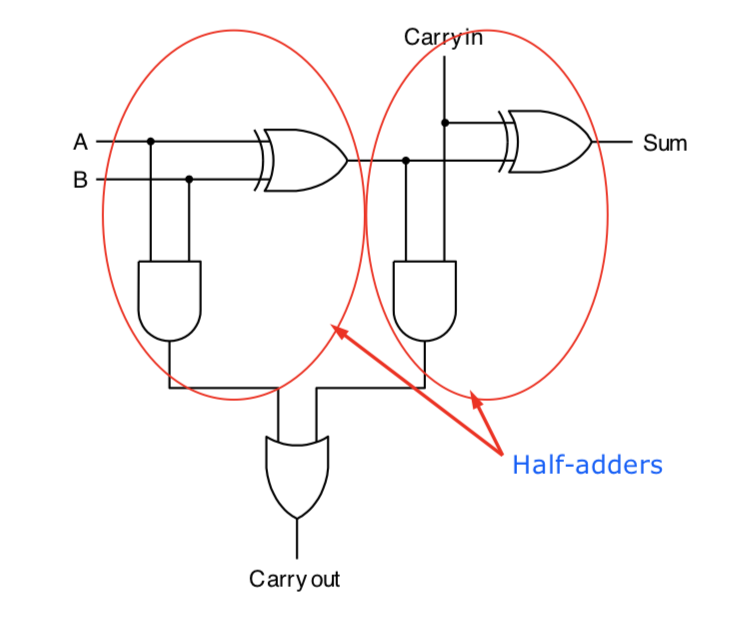
\includegraphics[width=0.8\linewidth]{fulladder}	
\end{figure}


\subsection{Binary Adder}
Can cascade full adders to make binary adder. This is a \textbf{ripple-carry adder}.
\begin{figure}[H]
	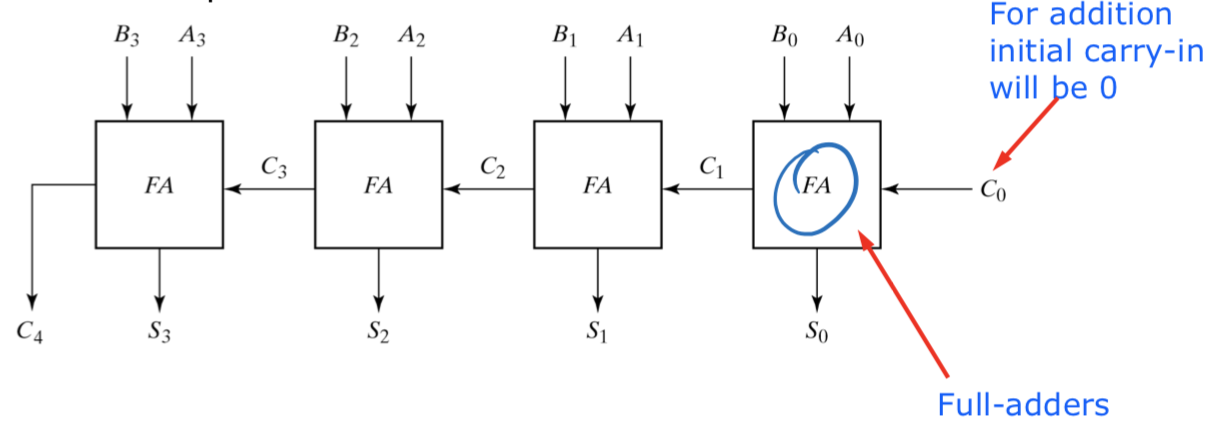
\includegraphics[width=0.8\linewidth]{binaryadder}	
\end{figure}



%\begin{circuitikz}
%	\draw (1, -2) node [and port,rotate=-90] (and1) {};
%	\draw (5, -2) node [and port,rotate=-90] (and2) {};
%	\draw (3, -4) node [or port,rotate=-90] (or1) {};
%	\draw (and1.out) |- (or1.in 2);
%	\draw (and2.out) |- (or1.in 1);
%	
%	\draw (3, 0.5) node [xor port] (xor1) {};
%	
%	\draw (0, 0) node (a) {A};
%	\draw (0, 1) node (b) {B};
%	
%	\draw (a) -| (and1.in 1);
%	\draw (a) -| (xor1.in 2);
%	\draw (b) -| (and1.in 2);
%	\draw (b) -| (xor1.in 1);
%\end{circuitikz}

\section{Synchronisation}
\subsection{Clock Synchronisation}
\begin{itemize}
	\item The problem with clocks in DS
	\item Physical clocks
	\item clock synchronisation algorithms:
	\subitem network time protocol (NTP)
	\subitem the berkeley algorithm
	\subitem clock synchronisation in wireless networks	
\end{itemize}

\subsubsection{Physical Clocks}
\begin{itemize}
	\item Sometimes we need the exact time in DS
	\item \textbf{Universal Coordinated Time (UTC)}
	\begin{itemize}
		\item Based on the number of transactions per second of the Cesium 133 atom
		\item At present, the real time is taken as the average of approx. 50 Cesium clocks around the world (International Atomic Time - TAI)
		\item Introduces a leap second from time to time to compensate that days are getting longer
	\end{itemize}
	\item UTC is broadcast through short wave radio and by satellite. Satellites can give an accuracy of about $\pm$ 0.5ms	
\end{itemize}

\subsubsection{Clock Synchronisation Algorithms}
\begin{itemize}
	\item Suppose we have a distributed system with a UTC receiver somewhere in it we still have to distribute its time to each machine
	\item Assumptions:
	\begin{itemize}
		\item Every machine has a timer that generates an interrupt $H$ times per second
		\item There is a clock in machine $p$ that \textbf{ticks} on each timer interrupt. Denote the value of that clock by $C_p(t)$, where $t$ is UTC time
		\item Ideally, we have that for each machine $p$, $C_p(t)=t$ or, in other words, $\frac{dC}{dt}=1$	
	\end{itemize}
\end{itemize}
If $\frac{dC}{dt}>1$, fast clock. If $\frac{dC}{dt} = 1$, perfect clock. If $\frac{dC}{dt} < 1$, slow clock.

\subsection{Network Time Protocol (NTP)}
\begin{itemize}
	\item The Network Time Protocol (NTP) was developer to synchronise clocks across DS
	\item NTP achieves accuracy of between 1 and 50 ms
	\item NTP servers are divided into strata reflecting the accuracy of their clocks
	\item The most accurate servers are referred to as stratum-1 (and typically have direct access to a reference clock)
	\item NTP operates pair-wise between servers	
\end{itemize}

\subsection{The Berkeley Algorithm}
\begin{itemize}
	\item Berkeley algorithm uses averaging approach to correct clocks (so doesn't need WWW receiver)
	\item Time daemon's clock must be manually set (periodically)
	\item New time is calculated as follows:
	\begin{itemize}
		\item daemon announces its time to each node on the network
		\item nodes report how far ahead/behind their clocks are
		\item daemon calculates new time based on average of reported values
		\item daemon tells each node how to adjust its clock
	\end{itemize}
\end{itemize}

\subsection{Wireless Networks}
Clock synchronisation in wireless networks is problematic because:
\begin{itemize}
	\item Nodes cannot always contact one another
	\item Nodes are resource-constrained	
\end{itemize}
Reference Broadcast Synchronisation (RBS) designed for wireless sensor networks
\begin{itemize}
	\item offers network internal synchronisation (not necessarily to UTC time)
	\item sender broadcasts reference message with timestamp
	\item receivers record difference between reference message timestamp and their own clock
	\item receivers store time offset (calculated using simple linear regression algorithm) for each sender
\end{itemize}

\subsection{Logical Clocks}
\begin{itemize}
	\item The order in which events occur in the DS is often more important than the time that they occurred
	\item The order of events can be established using logical clocks	
\end{itemize}

\subsubsection{Lamport's Algorithm}
\begin{itemize}
	\item Events in the DS can be ordered using Lamport's \textbf{happened-before} relation
	\item The \textbf{happened-before} relation on the set of events in a DS is the smallest relation satisfying:
	\begin{itemize}
		\item if $a$ and $b$ are events in the same process, and $a$ occurs before $b$, then $a\rightarrow b$ is true
		\item if $a$ is the event of a message being sent by one process, and $b$ is the receipt of that message in another process, then $a \rightarrow b$ is also true
	\end{itemize}
	\item This relation is transitive:	
	\subitem $a\rightarrow b$ and $b\rightarrow c$, then $a\rightarrow c$
	\item In Lamport's logical clock algorithm:
	\begin{itemize}
		\item each event $a$ has an associated time $C(a)$ based on the local clock
		\item between any two events, the clock must tick at least once (i.e. no two events ever occur at the same time)
		\item messages carry their sending time according to the sender's clock e.g. $C(b)$
		\item when a message is received, its time is compared against the local clock. If the local clock is less than $C(b)$, \textbf{it is set to $C(b)+1$}
	\end{itemize}
	\item Events occurring in processes that do not interact (even indirectly through third parties) are said to be concurrent
	\item Nothing can be said about the order of concurrent events
	\item For example:
	\begin{itemize}
		\item Events $x$ and $y$ occur in two different processes (that do not interact at all)
		\item The happened-before relation cannot be applied as $x$ and $y$ are concurrent
		\item This means that $x\rightarrow y$ is not true, and $y\rightarrow x$ is not true
	\end{itemize}
\end{itemize}

\subsubsection{Vector Clocks}
\begin{itemize}
	\item Lamport's algorithm ensures that if the happened-before relation exists between events $a$ and $b$, then $C(a) < C(b)$
	\item But if $C(c) < C(d)$, Lamport's algorithm doesn't guarantee that $c$ happened before $d$
	\item The problem is that Lamport's algorithm does not capture \textbf{causality}
	\item Causality can be captured using vector clocks
	\item The vector clock for an event $a$ is signified by $VC(a)$
	\item For two events, $a$ and $b$, if $VC(a) < VC(b)$, then event $a$ causally precedes event $b$
	\item To construct a vector clock, each process $P_i$ maintains a vector $VC_i$
	\subitem $VC_i[i]$ is the value of the logical clock at $P_i$
	\subitem If $VC_i[j] = k$, $P_i$ knows that at least $k$ events have occurred at $P_j$
	\item For every event that occurs at $P_i$ the vector value $PC_i[i]$ is incremented by one
	\item A process' vector is piggybacked onto all messages sent by that process
	\item Every time a message is received, the recipient process updates its own vector ($VC_r$)
	\item If we assume the message vector is $VC_m$, the update is performed by setting $VC_r[k] = MAX(VC_r[k], VC_m[k])$ for each $k$
	\item The issue of total ordering and causal ordering of messages by the communication system is controversial
	\item Total or causal ordering can also be provided in the application (\textbf{end-to-end} argument)	
\end{itemize}

\subsection{Mutual Exclusion}
\begin{itemize}
	\item Processes in a distributed system may want exclusive access to a shared resource
	\item A mutual exclusion mechanism is required to prevent corruption (or inconsistent updates) of that resource
	\item How to achieve mutual exclusion in DS?	
\end{itemize}

\subsubsection{A Centralised Algorithm}
\begin{itemize}
	\item Coordinator process enforces mutual exclusion over resource
	\item Processes must ask coordinator for permission to access resource
	\item Benefits of centralised approach:
	\begin{itemize}
		\item easy to implement
		\item low message overhead
		\item fair (access requests are processed in order)
	\end{itemize}
	\item Drawbacks:
	\begin{itemize}
		\item coordinator is a single point of failure
		\item coordinator can be performance bottleneck
	\end{itemize}
\end{itemize}

\subsubsection{Distributed, with no topology imposed (by Ricart and Agrawala)}
\begin{itemize}
	\item A process wanting to access a shared resource sends a message to all other processes. The message contains:
	\begin{itemize}
		\item the requested resource's name
		\item the requesting process' process id
		\item the requesting process' logical time
	\end{itemize}
	\item Recipients of the message follow one of three behaviours. If the recipient:
	\begin{itemize}
		\item doesn't want the resource, it sends back OK
		\item currently holds the resource, then it checks if the logical time in the message is less than its own logical time. If so, it sends back OK. If not, it queues the message and sends back nothing.
	\end{itemize}
	\item To access the shared resource, a process must receive an OK from all other processes
	\item When a process is finished with a resource it:
	\begin{itemize}
		\item sends OK messages to processes in its queue
		\item deletes its queue
	\end{itemize}
	\item Benefits of approach:
	\begin{itemize}
		\item solution is fair
		\item does not need a single coordinator
	\end{itemize}
	\item Drawbacks
	\begin{itemize}
		\item all processes are involved in all decisions (one slow process slows down others)
		\item large number of messages required
		\item single point of failure replaced with $n$ points of failure
		\item processes must have accurate group membership list
	\end{itemize}	
\end{itemize}


\subsubsection{Distributed, using a ring topology}
\begin{itemize}
	\item Uses a logical ring to order processes
	\item Processes can only access the shared resource while in possession of a token
	\item The token is passed on to the next node in the ring if:
	\begin{itemize}
		\item the current token holder does not want to access the shared resource
		\item if the token holder is finished accessing the shared resource
	\end{itemize}
	\item The token circulates around the ring in one direction
	\item Benefits of this approach:
	\begin{itemize}
		\item algorithm is simple
	\end{itemize}
	\item Drawbacks:
	\begin{itemize}
		\item token must be regenerated if lost
		\item crashed processes can stop circulation of token
		\item potentially have to wait for every other process to use token before it is your turn
	\end{itemize}	
\end{itemize}

\end{multicols}
\begin{table}[H]
	\centering\caption{Comparison of Algorithms}
	\begin{tabular}{l|p{5cm}p{5cm}l}
		\textbf{Algorithm} & \textbf{Messages per entry/exit} & \textbf{Delay before entry (in message times)} & \textbf{Problems} \\\hline
		Centralised & 3 & 2 & Coordinator crash\\
		Distributed & $2(n-1)$ & $2(n-1)$ & Crash of any process\\
		Token ring & $1$ to $\infty$ & $0$ to $n-1$ & Lost token, process crash	
	\end{tabular}
\end{table}
\begin{multicols}{2}

\subsection{Election Algorithms}
\begin{itemize}
	\item Many distributed algorithms require that one of the processes acts as a coordinator
	\item An election is used to dynamically select coordinator
	\item Election algorithms needed so that at the end of the election all processes agree on coordinator
	\item Common election algorithms are:
	\begin{itemize}
		\item the Bully Algorthm
		\item a Ring Algorithm
	\end{itemize}
	\item Different algorithms needed for:
	\begin{itemize}
		\item Wireless network environments
		\item Large-scale distributed systems
	\end{itemize}	
\end{itemize}

\subsubsection{The Bully Algorithm}
\begin{itemize}
	\item When process $P$ notices coordinator is non-responsive, it initiates an election
	\item Election conducted as follows:
	\begin{enumerate}
		\item $P$ sends an ELECTION message to all processes with higher process number
		\item If no one responds, $P$ wins the election and becomes coordinator
		\item If one of the higher-ups answers, it takes over. $P$'s job is done
	\end{enumerate}	
\end{itemize}

\subsubsection{A Ring Algorithm}
\begin{itemize}
	\item Assumes processes are logically ordered (each node knows its successor in ring)
	\item When process $P$ notices coordinator is non-responsive, it initiates election
	\item Election conducted as follows:
	\begin{itemize}
		\item $P$ sends ELECTION message (containing $P$'s process num) to successor
		\item Recipients add own process num to message and pass to  their successor
		\item Message gets back to $P$, who changes message type to COORDINATOR
		\item COORDINATOR message circles ring again
		\item Process with highest process num in COORDINATOR message becomes coordinator
	\end{itemize}	
\end{itemize}

\subsubsection{for Wireless Environments}
\begin{itemize}
	\item Previously described election algorithms need:
	\subitem reliable message passing
	\subitem stable network topology
	\item These aren't always present in wireless environments
	\item The following election protocol for wireless environments attempts to overcome these problems
	\item Node that calls election becomes \textbf{source node}
	\item Source node sends ELECTION message to all neighbours
	\item The first time a node receives ELECTION message it:
	\subitem marks sender as parent
	\subitem forwards ELECTION message to all its neighbours
	\item Subsequent ELECTION messages (not from parent) are acknowledged only
	\item Nodes wait a set time for acknowledgements from neighbours, before sending own acknowledgement to parent
	\item Acknowledgements contain information on the resource capacities of the node's best neighbour (e.g. battery power)
	\item The source node uses the acknowledgement information to select the coordinator	
\end{itemize}

\subsubsection{for Large-Scale Systems}
\begin{itemize}
	\item Previous algorithms select one node only
	\item Large-scale systems may require many local coordinators (e.g. peer-to-peer networks superpeers keep index of content on neighbours to speed searches)
	\item Superpeers should:
	\begin{itemize}
		\item offer regular nodes low-latency access
		\item be evenly distributed throughout network
		\item exist in predefined proportion to regular nodes
		\item serve no more than a set number of regular nodes
	\end{itemize}
	\item Two approaches for selecting superpeers:
	\subitem using a Distributed Hash Table (DHT) identifier
	\subitem using repulsion forces
	\item Distributed Hash Table identifier:
	\begin{itemize}
		\item fraction of DHT identifier space is reserved for superpeers
		\item reserve the first (i.e. leftmost) $k$ bits to identify superpeers
		\item need $N$ superpeers: use \textit{ceil(log2(N))} bits of any \textbf{key} to identify these nodes
	\end{itemize}
	\item Repulsion forces approach:
	\begin{itemize}
		\item $n$ tokens spread across peer-to-peer overlay
		\item each node holding a token learns about other token-holders
		\item each token is ``repulsed'' by nearby tokens (token holder sends token to another peer if too many tokens nearby)
		\item tokens passed around network until tokens spread evenly across network
		\item token must be held by a node for a set time period before node can become superpeer
	\end{itemize}	
\end{itemize}


\chapter{Seminar Slides}
\input{slides1}
\input{slides2}
% !TeX spellcheck = en_US
% !TeX root = notes.tex
\section{Solidity: Ethereum's Smart Contract Language}
\begin{itemize}
	\item Statically-typed programming language
	\item Compiles to bytecode which is run on the EVM
	\item Every operation (OP\_CODE) in the bytecode costs gas, this makes sure that smart contracts cannot run forever on the Turing Complete EVM
	\item A smart contract, in the case of Solidity, is a collection of code (the functions of the smart contract) and data (the state of the smart contract), which resides at a specific address on the Ethereum blockchain
\end{itemize}
\input{slides4}
\input{slides5}
\input{slides6}
\input{slides7}
\input{slides8}
\input{slides9}
\input{slides10}
\input{slides11}
\input{slides12}
\input{slides13}

\chapter{Paper Summaries}
\input{paper20}
\input{paper21}
\input{paper22}
\input{paper23}
\input{paper24}
\input{paper25}
\input{paper26}
\input{paper30}
\input{paper31}
\input{paper32}
\input{paper33}
\input{paper34}
\input{paper35}
\input{paper36}
\input{paper37}
\input{paper38}
\input{paper39}
\input{paper40}
\input{paper41}
\input{paper42}
\input{paper43}
\input{paper44}
\input{paper45}
\input{paper46}
\input{paper47}
\input{paper48}
\input{paper49}
\input{paper50}

\chapter{Do you need a Blockchain?}
\begin{itemize}
	\item Essentially Blockchain is only suitable for any system that requires a database or someway to store data, multiple writers (having only one writer would better suit using a regular database as better throughput) and no Trusted Third Party (TTP) that can always be relied on for writing. Otherwise don't use blockchain
	\item Types of Blockchain (Private/Public $\rightarrow$ Reader, Permissioned/Permissionless $\rightarrow$ Centralized)
	\begin{itemize}
		\item Permissionless Blockchain
		\item Public Permissioned Blockchain
		\item Private Blockchain
	\end{itemize}
\end{itemize}
\section{What are some examples where a blockchain would be necessary?}
\begin{description}
	\item[DOAs (Decentralized Autonomous Organizations)] CAN be useful, although they likely wouldn't need to use a full fledged permissionless blockchain in most cases
	\item[Finance (interbank payments):] Multiple parties that don't trust each other that need high number of readers but not necessarily high throughput. Although this would certainly still use the central bank only has a TTP to authorize other banks and be a permissioned blockchain, public vs private is a matter of public opinion
	\item[IoT:] Payment systems between machines, smart cars charging at electric charging stations, small devices requiring data processing from untrusted server. However, sensors play a huge role and thus need to be trusted by all parties, thus this depends on a case by case basis
	\item[Voting:] Multiple parties not trusting the outcome as valid, need a mechanism that is able to verify votes, where they came from, only one vote spent, cannot forge votes or create new ones. Essentially system requires public verifiability as many mutually untrusted parties exist
	\item[Smart Contracts:] Well suited as no need for TTP. Either permissioned or permissionless
	\item[Multi-party Trade:] Exchanging digital goods without trusted dispute mediator, physical goods still require TTP to handle disputes
	\item[Proof of ownership:] In the case of patenting, it would be handy to have a verifiable record, however this does not always fully prove ownership
\end{description}
\section{Properties of Distributed Ledgers vs Centralized Systems}
\begin{itemize}
	\item Public verifiability
	\item Transparency
	\item Privacy
	\item Integrity
	\item Redundancy
	\item Trust Anchor
\end{itemize}

\chapter{Past Exams}
\section{2017 Sample}

\subsection{Question 1}
Alice, Bob, Charlie and Debbie use Shamir's method to implement a (2, 4)-threshold secret sharing scheme to share the secret $K$. Computations are done in GF(7), i.e. modulo 7. Bob's and Charlie's shares are as follows:\\
Bob: $(x_B,y_B)=(3,5)$\\
Charlie: $(x_C,y_C)=(5,4)$\\
Compute the shared secret $K$\\\\

\begin{align*}
	5 &= 3m+c \tag{Bob}\\
	\frac{5-c}{3} &= m\\
	\frac{5}{3} - \frac{1c}{3} &= m\\
	\frac{12}{3} - \frac{15c}{3} &= m\\
	4 - 5c &= m\\
	m &= 4-5c\\
	4 &= 5m+c \tag{Charlie}\\
	4 &= 5(4-5c)+c\tag{Sub Bob into Charlie}\\
	4 &= 20 - 25c + c\\
	4 &= 20 - 24c\\
	4 &= 6 - 3c\\
	-2 &= -3c\\
	2 &= 3c\\
	\frac{2}{3} &= c\\
	\frac{30}{3} &= c\\
	10 &= c\\
	3 &= c
\end{align*}

\subsection{Question 3}
Blind Signatures are used to enable a user to verify the a set of information without knowing what that information is. This is used to maintain anonymity in cryptocurrencies where a coin will be blindly signed by the bank to ensure they can't trace payments. The RSA signature process uses a blind signature to get information signed without the singer knowing what they are signing.

\subsection{Question 4}
In a Shamir secret sharing scheme, the secret is the constant term $c$ of a polynomial of degree $4$. Computations are done in GF(991), i.e. modulo the prime 991. Suppose Alice, Bob and Susie have the following three shares: $(2,197),(4,874),(13,547)$. How many possibilities are there for the secret? How much information can be gained from the three shares? Explain your answer.\\\\

Because the polynomial is of degree 4, there is still one point of freedom which does not provide any additional knowledge of the curve. The only known information is that the secret lies somewhere between 0 and 991.

\subsection{Question 5}
Generate two valid shares for a secret $K=30$ in a (3, 4)-threshold secret sharing scheme (Blakely's method). Computations are done in GF(37). Explain the individual steps involved.\\\\

$$ y = m_1x^3 + m_2x^2 + m_3x + c$$
Share 1: $y = 5x^3 + 3x^2 + 10x + 30$
Random points: $(1,48), (2, 102), (10, 5430) \rightarrow (1, 11), (2, 28), (10, 28)$


\end{multicols*}
\end{document}
